\section{Øvelse 3}
\subsection{Opgave 1 - Four bit parallel adder}
\begin{enumerate}
	\item[1)]
Vi designer en 4 bit parallel adder i structural style ved hjælp af den dataflow-style four bit full adder, vi har lavet i øvelse 2 (se Kode \ref{lst:FaDataflowCode})


	\medskip
	\begin{lstlisting}[caption={Four bit parallel adder Structural VHDL kode},label={lst:4bitFaStructuralCode}]
	library ieee;
	use ieee.std_logic_1164.all;
	
	entity four_bit_full_adder is
	port (a: in std_logic_vector (3 downto 0);
	b: in std_logic_vector (3 downto 0);
	Cin: in std_logic;
	sum: out std_logic_vector (3 downto 0);
	Cout: out std_logic);
	
	end four_bit_full_adder;
	
	architecture structural of four_bit_full_adder is
	
	signal i1, i2, i3 : std_logic;
	begin
	full_ad1 : 	entity work.full_adder_dataflow port map (a => a(0), b => b(0), carry_in => cin, sum => sum(0), carry_out => i1 );
	full_ad2 : 	entity work.full_adder_dataflow port map (a => a(1), b => b(1), carry_in => i1, sum => sum(1), carry_out => i2 );
	full_ad3 : 	entity work.full_adder_dataflow port map (a => a(2), b => b(2), carry_in => i2, sum => sum(2), carry_out => i3 );
	full_ad4 : 	entity work.full_adder_dataflow port map (a => a(3), b => b(3), carry_in => i3, sum => sum(3), carry_out => Cout );
	
	end structural;
	\end{lstlisting}
	
\begin{figure}[H]
	\item[2)]
	Vi kan ved hjælp af RTL-viewer se, om vores full adders er forbundet korrekt:
	\centering
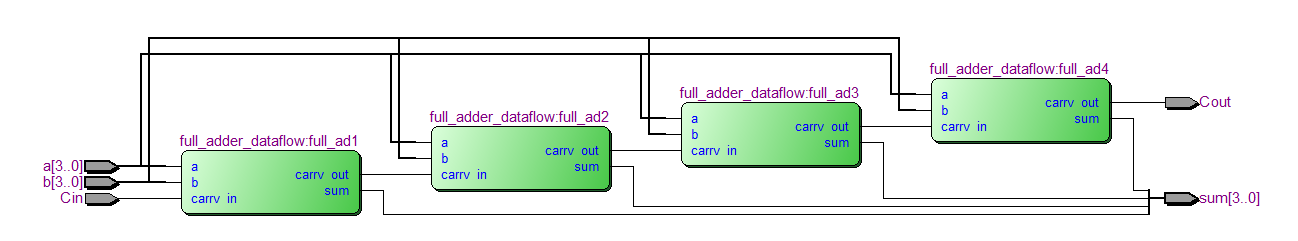
\includegraphics[scale=0.6]{pictures/Oevelse2/four_bit_full_adder_RTLview.jpeg}
\caption{Four bit parallel adder - Structural RTL view}
\label{fig:4bitFaBehavioralRTL}
\end{figure}

	\begin{figure}[H]
		\item[3)]
		Vi starter med at sætte bits til 00001111 samt cin 0 og får det forventede resultat:
		\centering
		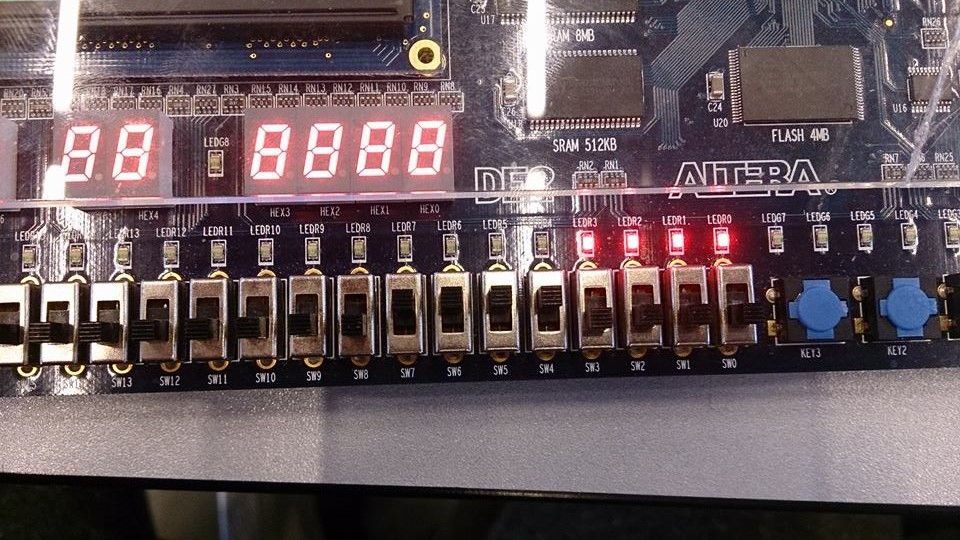
\includegraphics[scale=0.5]{pictures/Oevelse3/00001111_cin0.jpg}
		\caption{Four bit parallel adder - 00001111, cin=0}
		\label{fig:4bitFa00001111cin0}
	\end{figure}

	\begin{figure}[H]
Vi sætter nu bits til 11110000 samt cin 1 og får det forventede resultat:
		\centering
		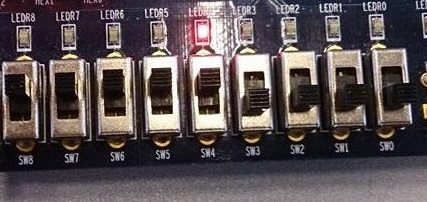
\includegraphics[scale=0.5]{pictures/Oevelse3/11110000_cin1.jpg}
		\caption{Four bit parallel adder - 11110000, cin=1}
		\label{fig:4bitFa11110000cin1}
	\end{figure}


	\begin{figure}[H]
			Vi sætter nu bits til 00010001 samt cin 1 og får det forventede resultat:
			\centering
			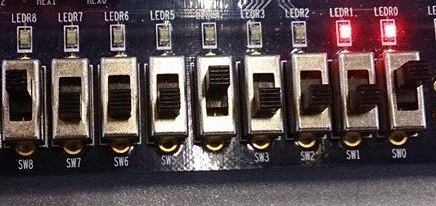
\includegraphics[scale=0.5]{pictures/Oevelse3/00010001_cin1.jpg}
			\caption{Four bit parallel adder - 00010001, cin=1}
			\label{fig:4bitFa00010001cin1}
		\end{figure}
		
\end{enumerate}
\newpage
\subsection{Opgave 2 - Four bit adder - using signed/unsigned logic}

\begin{enumerate}
	\item[1)]
	Vi laver en unsigned adder i dataflow style som vist på figur \ref{fig:4bitUnsignedAdder}. Da input og output skal være af std logic vector typen, og vi skal bruge + operatoren, bliver vi nødt til at konvertere til unsigned først. Se Kode \ref{lst:4bitUnsignedDataflowCode}\\
	
	\begin{figure}[H]
		\centering
		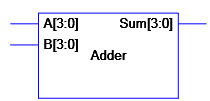
\includegraphics[scale=0.5]{pictures/Oevelse3/4bit_unsigned_adder.jpg}
		\caption{Four bit unsigned adder}
		\label{fig:4bitUnsignedAdder}
	\end{figure}
	
	\begin{lstlisting}[caption={Four bit unsigned adder Dataflow VHDL kode},label={lst:4bitUnsignedDataflowCode}]
	library ieee;
	use ieee.std_logic_1164.all;
	use ieee.numeric_std.all;
	
	entity unsigned_adder is
	port (a: in std_logic_vector (3 downto 0);
	b: in std_logic_vector (3 downto 0);
	sum: out std_logic_vector (3 downto 0));
	end unsigned_adder;
	
	architecture dataflow of unsigned_adder is
	begin
	
	sum <= std_logic_vector(unsigned(a) + unsigned(b));
	end dataflow;
	\end{lstlisting}
	
	\item[2)]
	Vi tester nu vores kode med en functional simulation:\\
	\begin{figure}[H]	
		\centering
		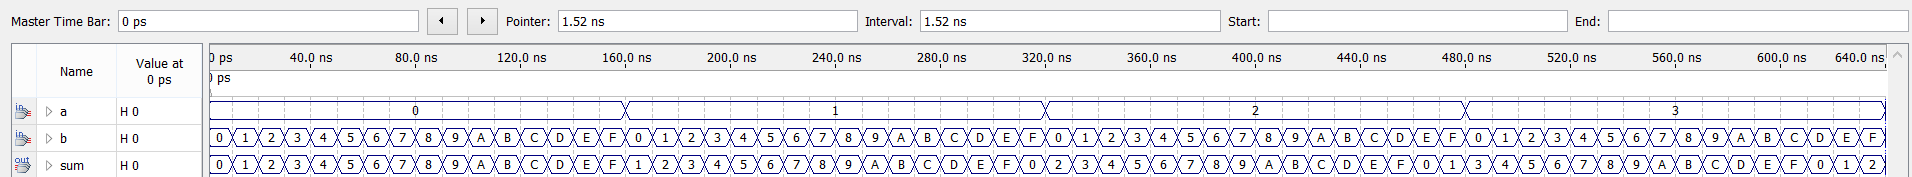
\includegraphics[scale=0.4]{pictures/Oevelse3/4bit_unsigned_adder_functional_simulation.jpeg}
		\caption{Four bit unsigned adder Functional simulation}
		\label{fig:4bitUnsignedAdderFuncSim}
	\end{figure}
\newpage
	\item[3)]
	Vi sætter nu bits til 1000 + 0100 og får det forventede resultat som det ses på Figur \ref{fig:4bitUnsignedAdder1100}\\
	\begin{figure}[H]
		
		\centering
		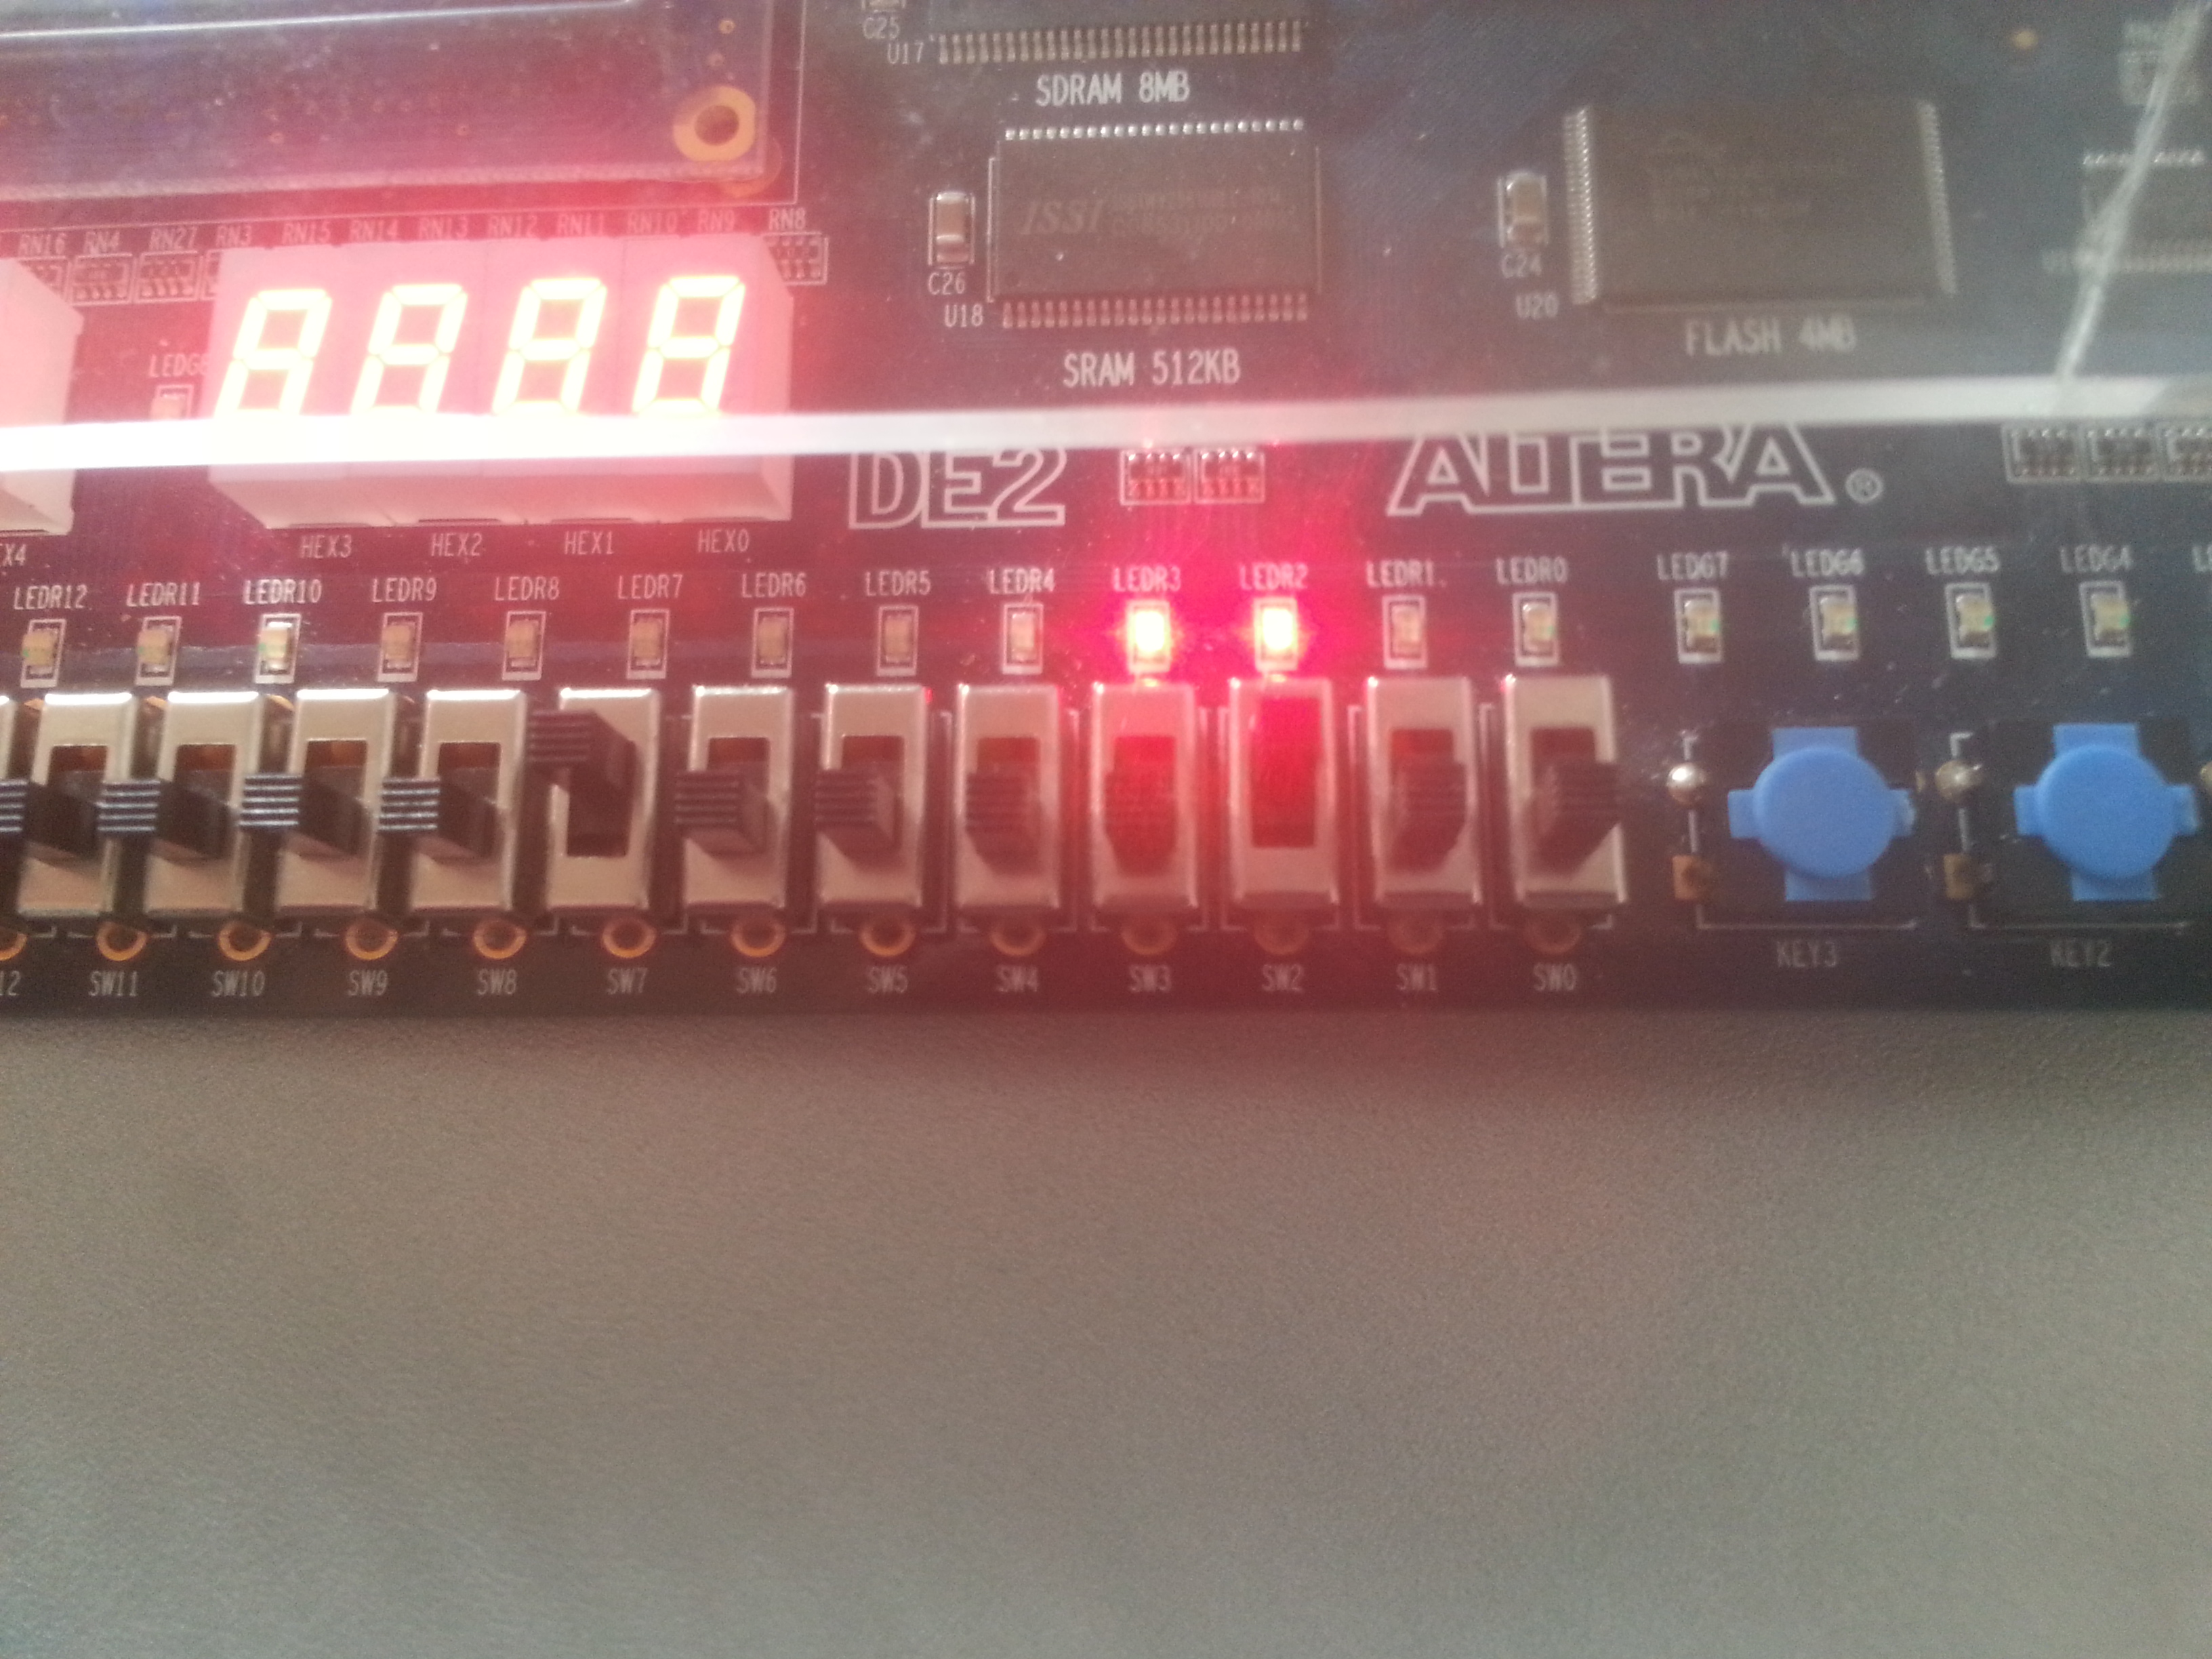
\includegraphics[width=0.8\textwidth]{pictures/Oevelse3/four_bit_unsigned_adder1.jpg}
		\caption{Four bit unsigned adder - 1000 + 0100}
		\label{fig:4bitUnsignedAdder1100}
	\end{figure}

	\item[4)]
	Vi ændrer nu koden så det bliver en signed adder som det ses i Kode \ref{lst:4bitsignedDataflowCode}. Vi tester det på vores DE2 board, og ser at der ingen forskel er på unsigned adderen og signed adderen som det ses på Figur \ref{fig:4bitSignedAdder1100}. Dette skyldes at selve bit'sne ikke er anderledes, men det er kun måden de skal tolkes på.
	
	\begin{lstlisting}[caption={Four bit signed adder Dataflow VHDL kode},label={lst:4bitsignedDataflowCode}]
	library ieee;
	use ieee.std_logic_1164.all;
	use ieee.numeric_std.all;
	
	entity unsigned_adder is
	port (a: in std_logic_vector (3 downto 0);
	b: in std_logic_vector (3 downto 0);
	sum: out std_logic_vector (3 downto 0));
	end unsigned_adder;
	
	architecture dataflow of unsigned_adder is
	begin
	
	sum <= std_logic_vector(unsigned(a) + unsigned(b));
	end dataflow;
	\end{lstlisting}
	
	\begin{figure}[H]
		
		\centering
		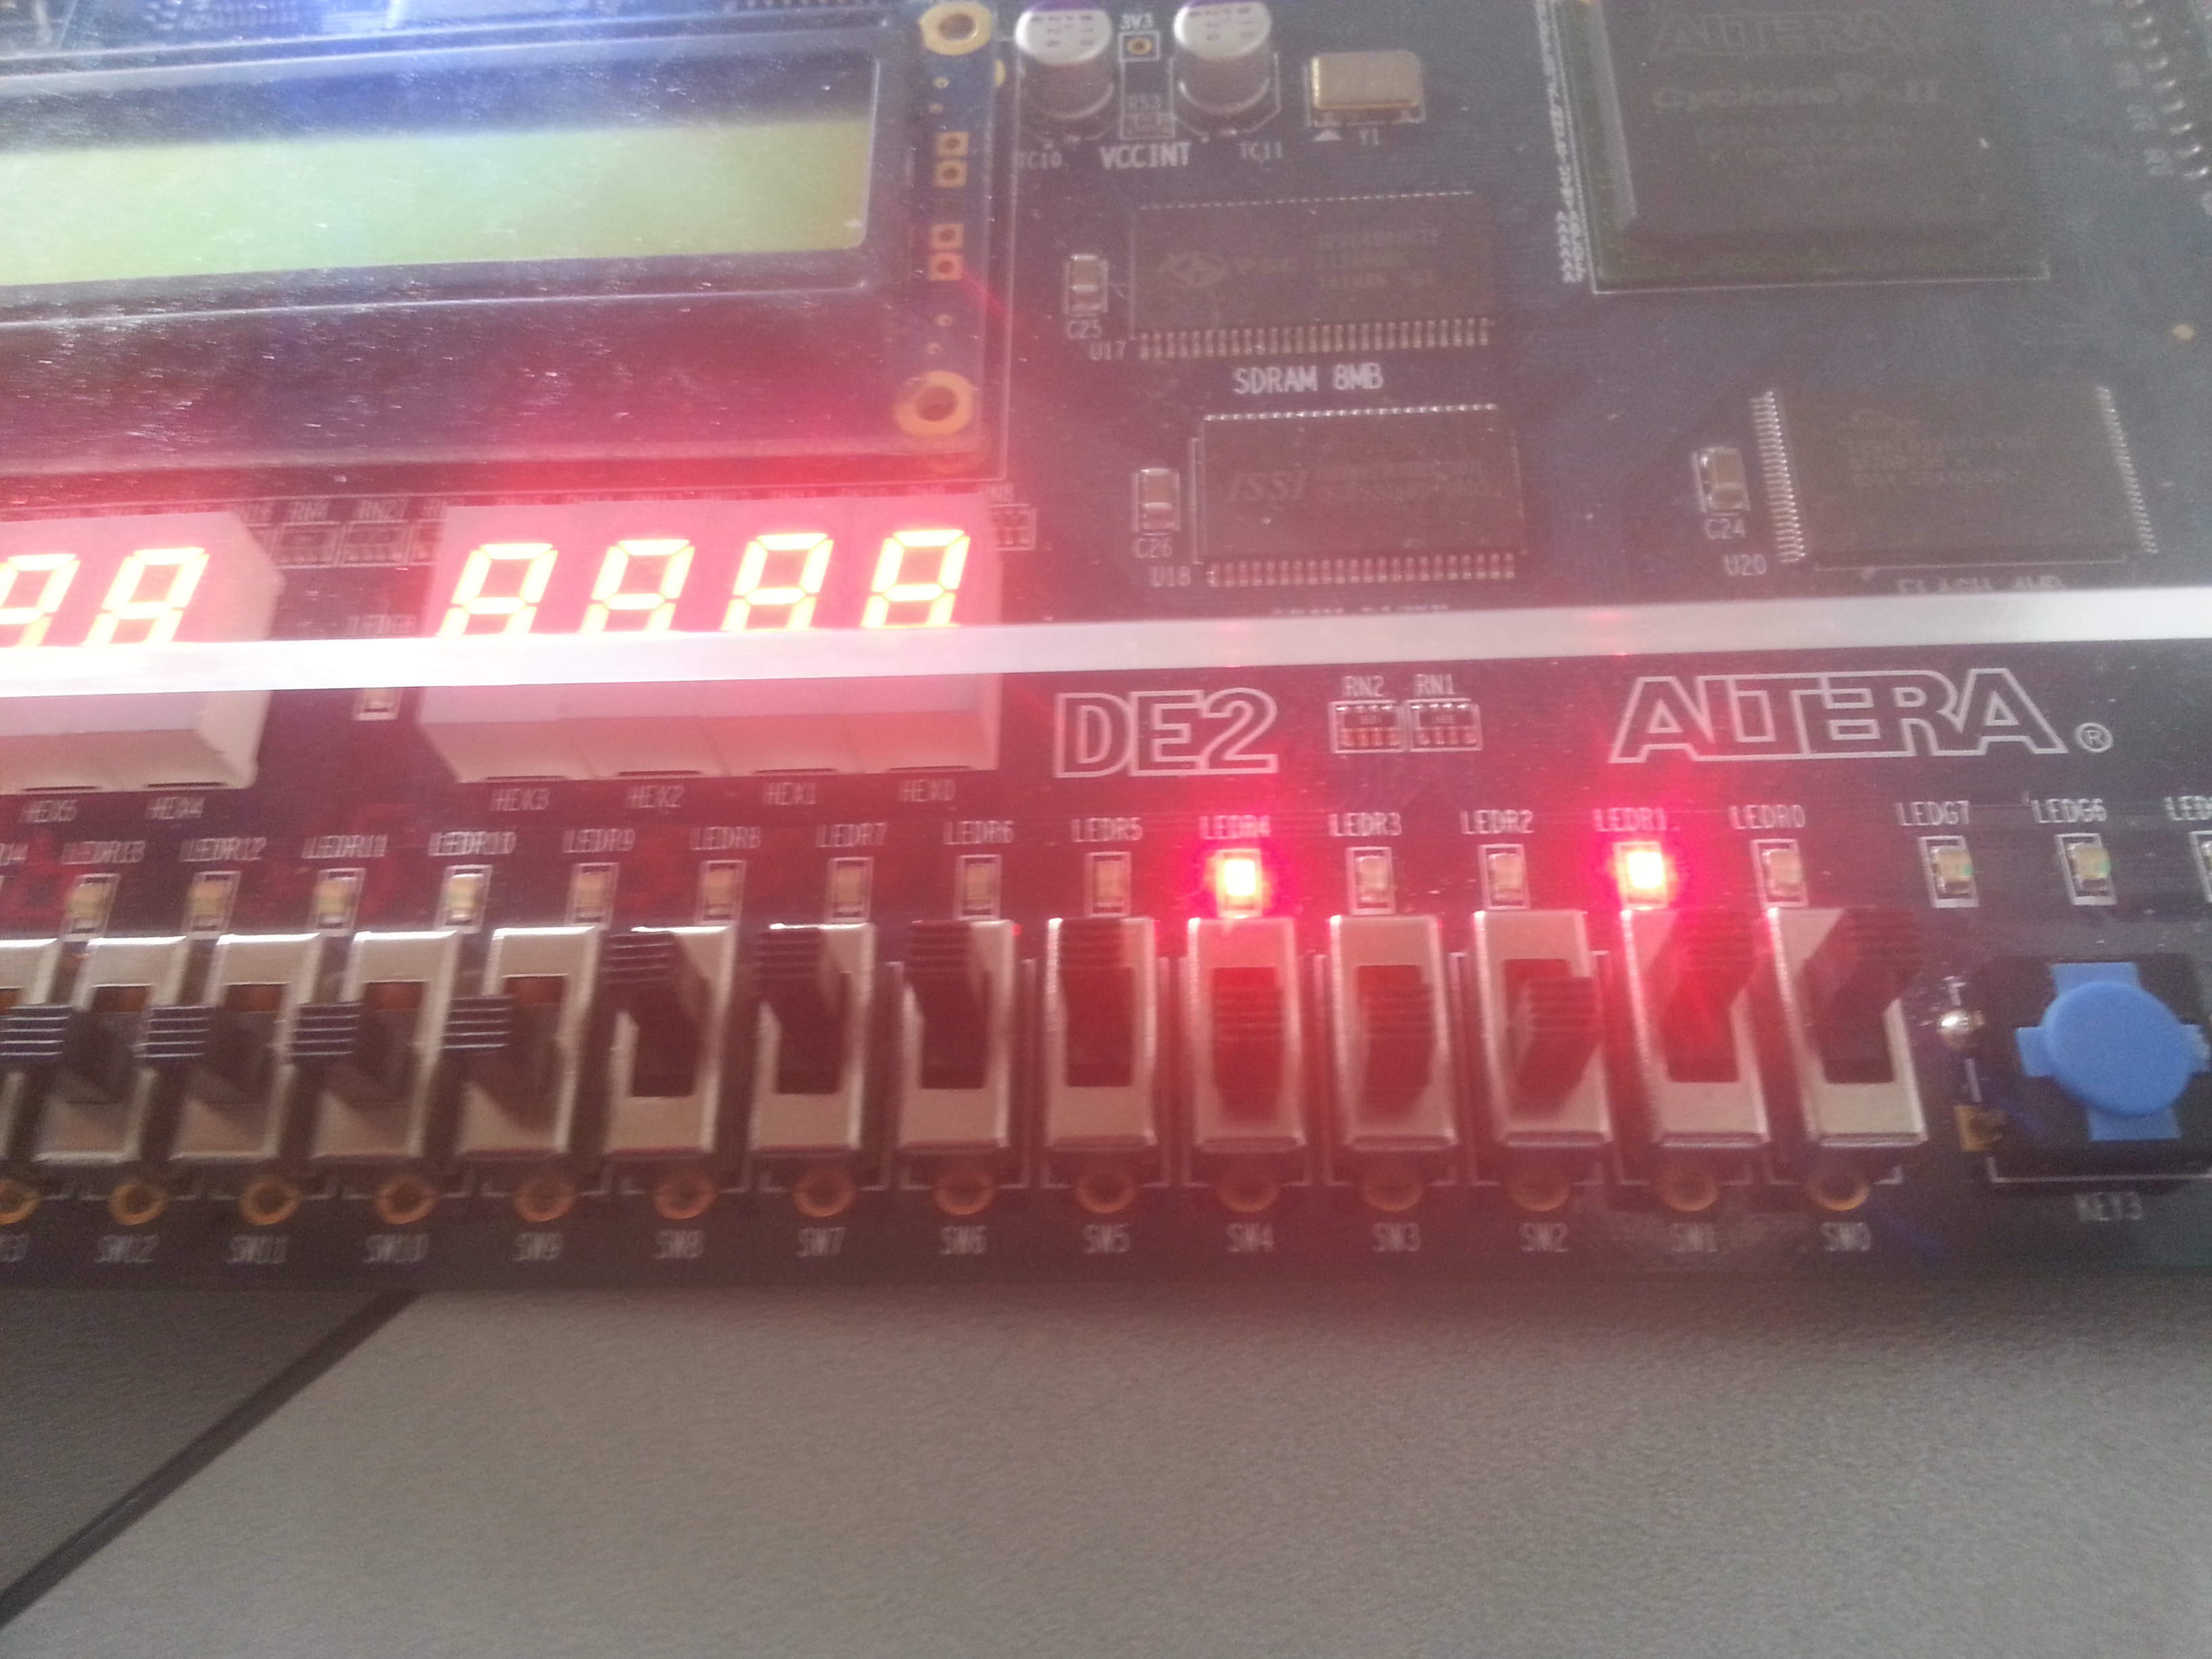
\includegraphics[width=0.8\textwidth]{pictures/Oevelse3/four_bit_signed_adder1.jpg}
		\caption{Four bit signed adder - 1000 + 0100}
		\label{fig:4bitSignedAdder1100}
	\end{figure}
\item[5)]
Vi laver nu vores unsigned adder om, så den også virker med et carry in, og leverer et carry out som vist på Figur \ref{fig:4bitUnsignedAdderCarry}. Vi benytter os af resize funktionen, samt laver nogle interne signaler, inden vi sender resultatet ud igen. Koden ses i Kode \ref{lst:4bitunsignedCarryDataflowCode}.
	\begin{figure}[H]
		\centering
		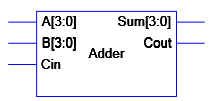
\includegraphics[scale=0.5]{pictures/Oevelse3/4bit_unsigned_adder_carry.jpg}
		\caption{Four bit unsigned adder with carry}
		\label{fig:4bitUnsignedAdderCarry}
	\end{figure}

	\begin{lstlisting}[caption={Four bit unsigned adder with carry Dataflow VHDL kode},label={lst:4bitunsignedCarryDataflowCode}]
	library ieee;
	use ieee.std_logic_1164.all;
	use ieee.numeric_std.all;
	
	entity unsigned_adder_carry is
	port (a: in std_logic_vector (3 downto 0);
	b: in std_logic_vector (3 downto 0);
	carry_in: in std_logic;
	carry_out : out std_logic_vector (0 downto 0);
	sum: out std_logic_vector (3 downto 0));
	end unsigned_adder_carry;
	
	architecture dataflow of unsigned_adder_carry is
	signal c : unsigned (3 downto 0);
	signal s : unsigned (4 downto 0);
	begin
	c <= "000" & carry_in;
	s <= resize(unsigned(a),5) + resize(unsigned(b),5) + resize(c,5) ;
	sum <= std_logic_vector(s(3 downto 0));
	carry_out <= std_logic_vector(s(4 downto 4));
	end dataflow;
	\end{lstlisting}

	\item[6)]
	Vi overfører vores adder til DE2 boardet. Her adderer vi 1110 + 0011 samt carry in = 1, og får det forventede resultat som ses på figur \ref{fig:4bitUnsignedAdderCarry10100}.
	\begin{figure}[H]
		\centering
		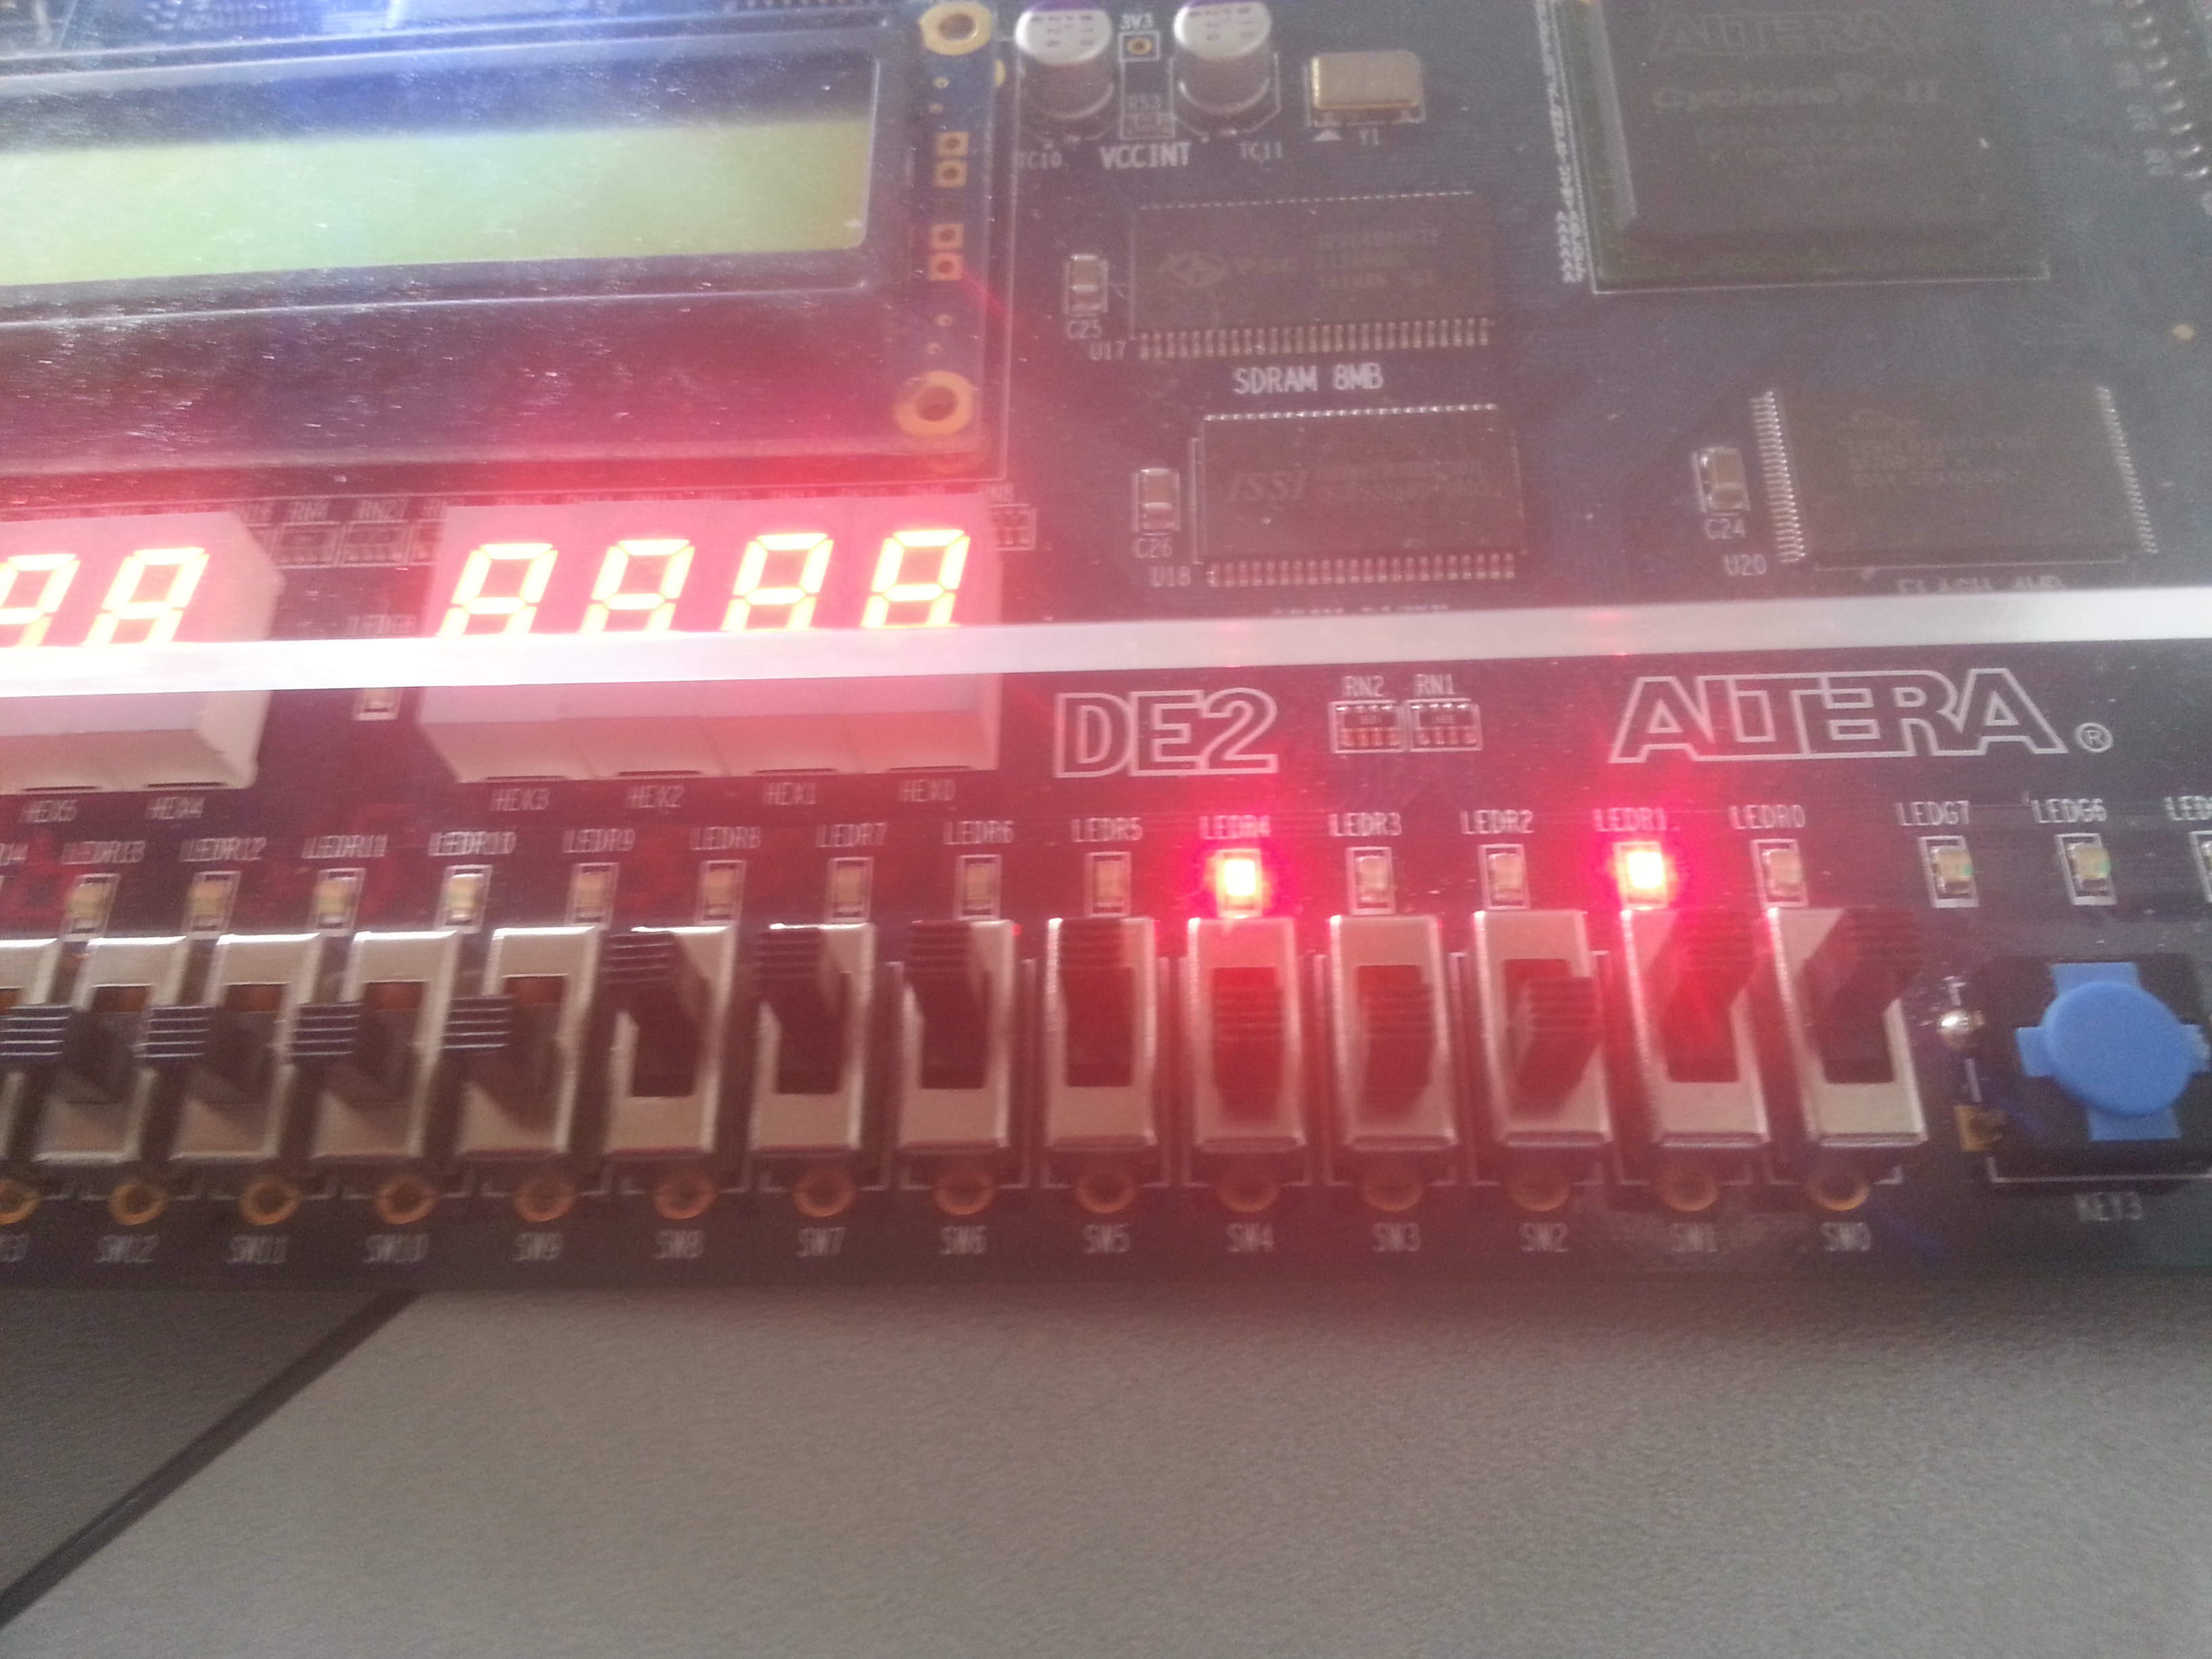
\includegraphics[width=0.8\textwidth]{pictures/Oevelse3/4bit_unsigned_adder_carry2.jpg}
		\caption{Four bit unsigned adder with carry}
		\label{fig:4bitUnsignedAdderCarry10100}
	\end{figure}
	
\end{enumerate}
\newpage
\medskip
\subsection{Opgave 3 - Concatenation}
\begin{enumerate}
	\item[1)]
		\begin{lstlisting}[caption={Concatenation kode},label={lst:ConcatenationCode}]
	library ieee;
	use ieee.Std_logic_1164.all;
	
	entity shift_div is
	port (a : in std_logic_vector(7 downto 0);
	a_shl,a_shr,a_ror: out std_logic_vector(7 downto 0));
	end shift_div; 
	
	architecture dataflow of shift_div is
	
	begin 
	a_shl <= a(6 downto 0) & '0';
	
	a_shr <= "00" & a(7 downto 2);
	
	a_ror <= a(2 downto 0) & a(7 downto 3);
	
	end dataflow ;

		\end{lstlisting}
	\item[2)]
Vi kan se på figur \ref{fig:concatenationRTL} fra RTL-viewer, at der ikke er nogen logiske elementer i kodestykket:
	\begin{figure}[H]
		\centering
		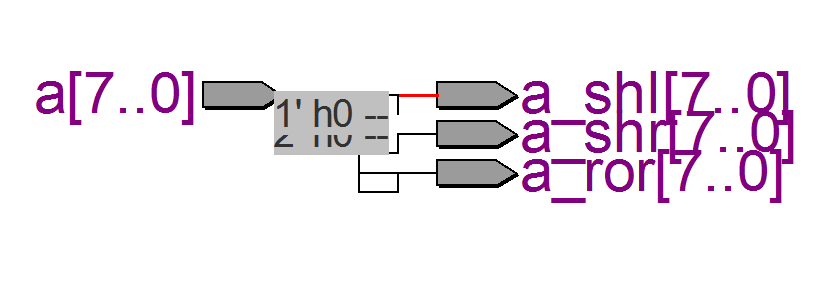
\includegraphics[scale=0.5]{pictures/Oevelse3/Concatenation_RTL.png}
		\caption{Concatenation RTL}
		\label{fig:concatenationRTL}
	\end{figure}

	
	\item[3)]
Vi overfører programmet til DE2-boardet. Inputtet a sættes som SW[7:0], output a-shl sættes til LEDR[7:0], a-shr sættes til LEDR[17:10] og a-ror sættes til LEDG[7:0]. Dette kan ses på figur \ref{fig:concatenation_DE2board}.

	\begin{figure}[H]
		\centering
		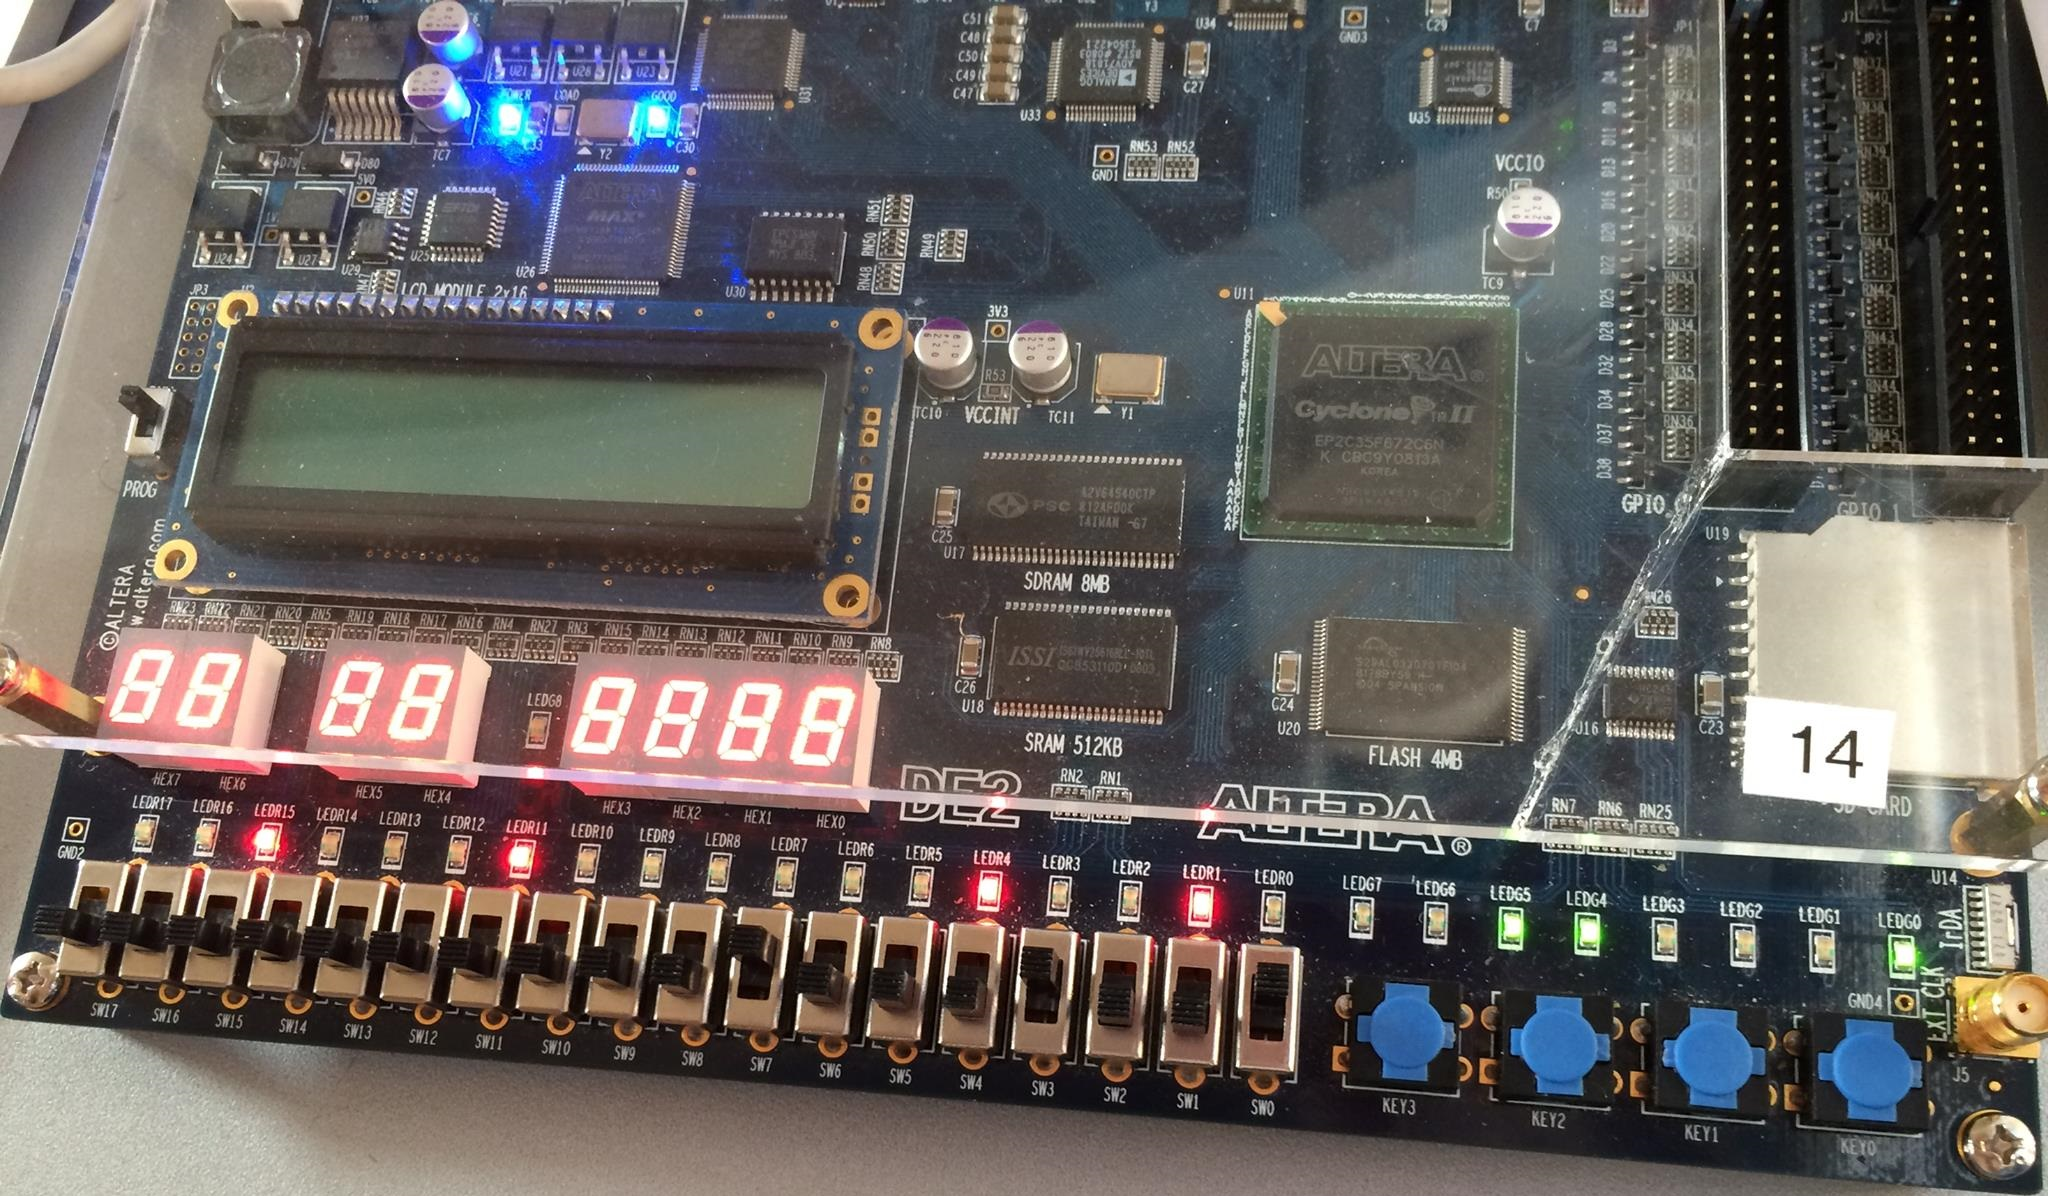
\includegraphics[scale=0.23]{pictures/Oevelse3/Concatenation_DE2board.jpg}
		\caption{Concatenation på DE2-board}
		\label{fig:concatenation_DE2board}
	\end{figure}

\end{enumerate}

\subsection{Opgave 4 - Subtype}
\begin{enumerate}
	\item[1)]
	Vi opskriver koden for en 4-bit subtractor som ses i kode \ref{lst:SubtractorCode}
	\begin{lstlisting}[caption={Subtractor kode},label={lst:SubtractorCode}]
	library ieee;
	use ieee.std_logic_1164.all;
	
	entity Subtypes is
	port (a,b : in std_logic;
	c  : out std_logic);
	end Subtypes;
	
	architecture dataflow of Subtypes is
	subtype bool is std_logic range '1' to 'Z';
	signal tmp : bool;
	begin 
	tmp<= 'U';
	c<= b and tmp;
	end dataflow;
		\end{lstlisting}
	\item[2)]
	
	Grunden til at vi får fejlen at U er udenfor rækkevidde ses på figur \ref{fig:stdulogicvalues} nedenfor:
	
		\begin{figure}[H]
			\centering
			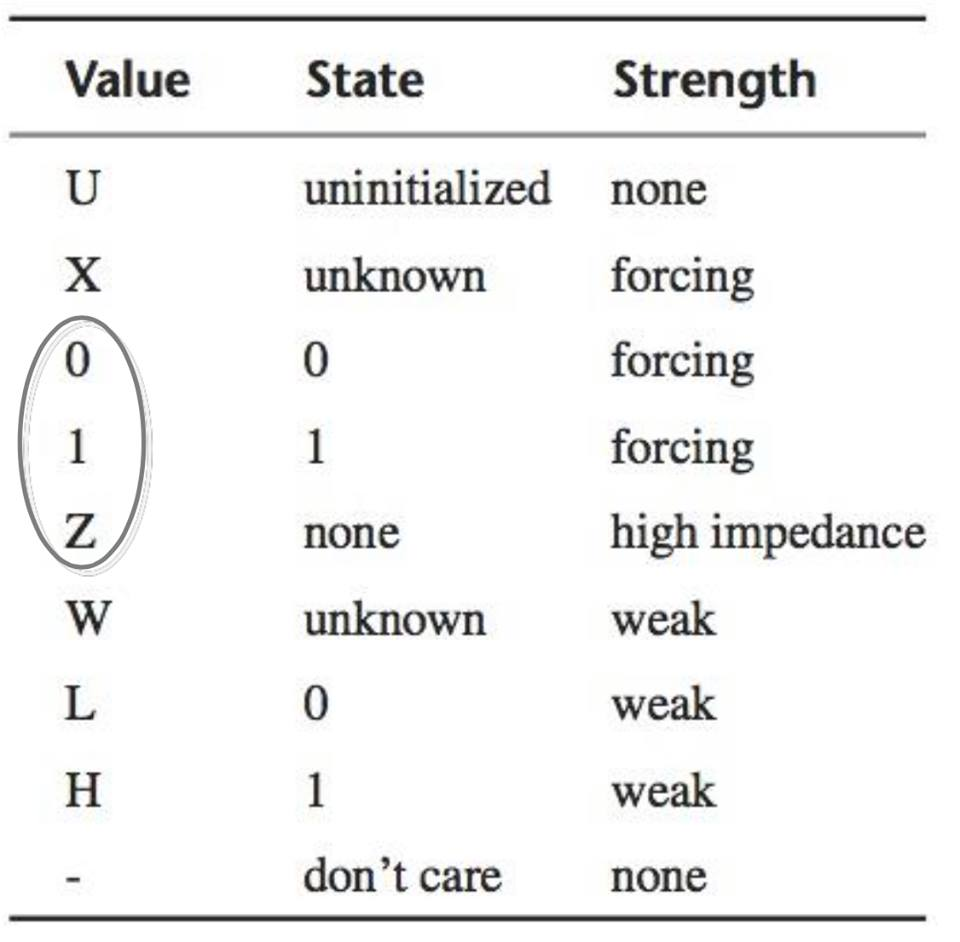
\includegraphics[scale=0.23]{pictures/Oevelse3/Oevelse4_01Z.jpg}
			\caption{Stater og styrker for std\_ulogic værdier}
			\label{fig:stdulogicvalues}
		\end{figure}
	
	
	Derfor retter vi til koden
	
	\begin{lstlisting}[caption={Rettet subtractor kode},label={lst:SubtractorCode2}]
library ieee;
use ieee.std_logic_1164.all;

entity Subtypes is
port (a,b : in std_logic;
c  : out std_logic);
end Subtypes;

architecture dataflow of Subtypes is
subtype bool is std_logic range 'U' to 'Z';
signal tmp : bool;
begin 
tmp<= 'U';
c<= b and tmp;
end dataflow;
	\end{lstlisting}	

	
\end{enumerate}


